%\chapter*{knx}

\section{Introduction to KNX}

KNX implements a specialized form of automated process control, dedicated to the needs of home
and building automation. KNX emerged from 3 leading standards:

\begin{itemize}
 \item EIB
 \item EHS
 \item BATIBUS
\end{itemize}


\begin{figure}
    \centering
    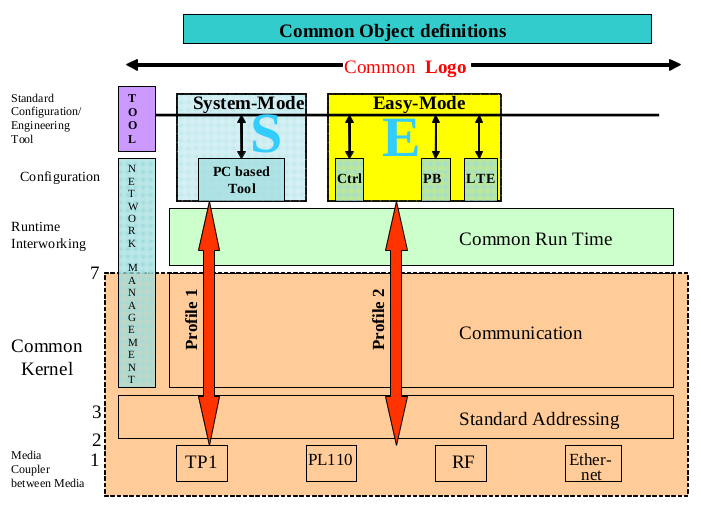
\includegraphics[width=0.8\textwidth]{figures/knx stack.png}
    \caption{The KNX Stack}
    \label{fig:knx_stack}
\end{figure}

\subsection{Datapoints}

Datapoints represent the process- and control variables of the system, and can be of
inputtype, outputtype, diagnostic data, parameters or others. To achieve interoperability,
Datapoints are grouped into functional blocks, implementing standardized datapoint types.

\section{KNX Layers}

The \textit{Open Systems Interconnection Model} OSI standardizes the communication between different, independent systems
by grouping the needed functions into 7 sublayers to provide interchangeability and abstraction. KNX implements this model, omitting 
layers 5 and 6, as shown in figure \ref{fig:knxlayers}. Data from applications are directly passed to the transport layer in a transparent way, and vice versa.

\begin{figure}
    \centering
    \includegraphics[width=0.8\textwidth]{figures/"knx vs iso layers".png}
    \caption{OSI Layer Model, compared to the KNX Model}
    \label{fig:knxlayers}
\end{figure}

\subsection{Physical Layer}

\begin{itemize}
 \item TP1 was inherited from EIB and is the basis medium, consisting of a twisted pair 
 cabeling. Data and power can be transmitted with one pair, so low-power devices can be
 fed over the bus. Data transfer is done asynchronously, with bidirectional, half-duplex
 communication and a datarate of 9600 bit/sec. TP1 uses collision avoidance, and allows
 all topologies beside rings. 
 
 Because this work is base on the TP1 - part of KNX only, this physical layer is explained
in more detail in the next chapter.

 \item PL110, which was also inherited from EIB, uses the power line for communications.
 The carrier uses spread frequency shift keying, also for bidirectional, half duplex 
 communication with a even lower data rate of 1200 bit/sec
 
 \item RF is used for short range wireless communication at 868,3 MHz. 

 \item IP Gateway FIXME
\end{itemize}

\subsubsection{TP1}

The accurate name for this medium is 'Physical Layer type Twisted Pair', with variants
PhL TP1-64 and PhL TP1-256, which is backward compatible to the former one.
\\*
\\*
The logical structure of the TP1 layer is shown in figure\ref{fig:tp1}
\\*
A logical '1' is regarded as the idle state of the bus, so the transmitter
of the MAU(Medium Access Unit) is disabled when sending a '1', so the analog signal on
the bus consists only of the DC part.
\\*A logical '0' is then defined as the voltage drop for a specified duration of t\textsubscript{active},
after which the voltage can increase over DC level, see figure\ref{fig:low}

\begin{figure}
    \centering
    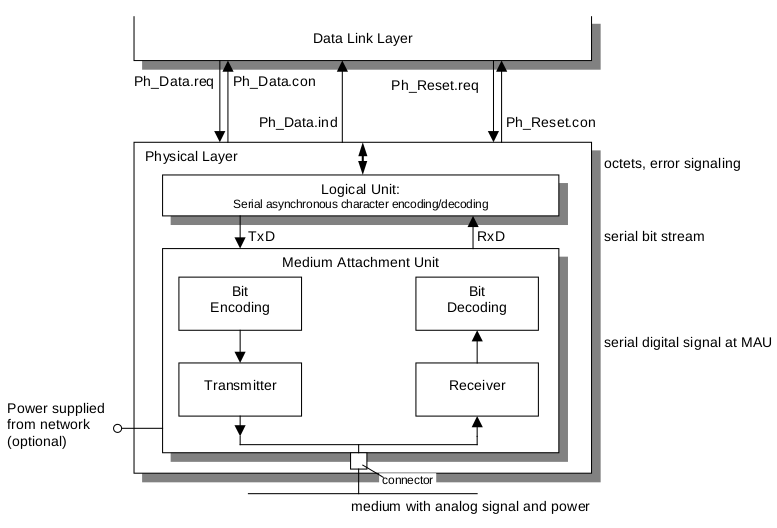
\includegraphics[width=0.5\textwidth]{figures/tp1-structure.png}
    \caption{Logical Structure of TP1}
    \label{fig:tp1}
\end{figure}

\begin{figure}
    \centering
    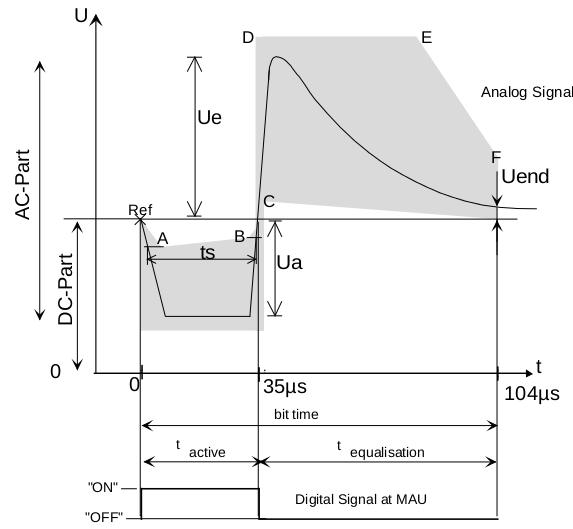
\includegraphics[width=0.5\textwidth]{figures/tp1-low.png}
    \caption{Logical 0}
    \label{fig:low}
\end{figure}

TP1 implements CSMA/CA, so devices will listen to the bus and should only begin sending
when the bus is idle. In the case of a simultaneous transmission start, a logical '1' of one
device will eventually be overwritten by a logical '0' of the other device. The overruled
sender will detect this by continuously checking the state of the bus and has to stop 
transmission.

\subsection{Data Link Layer}

\begin{figure}
    \centering
    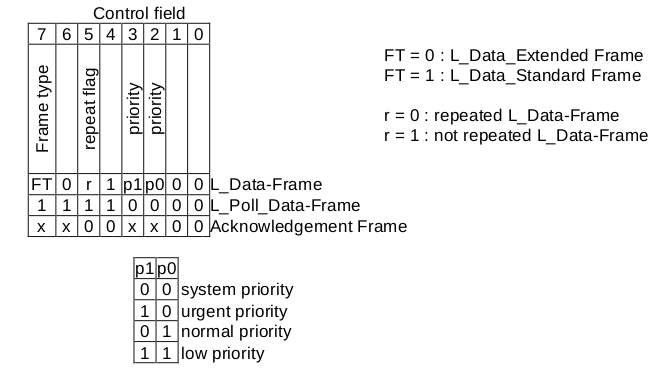
\includegraphics[width=0.5\textwidth]{figures/controlfield.png}
    \caption{Control Field}
    \label{fig:ctrlfield}
\end{figure}

There are defines 3 frame formats which are allowed, each  with the MSB sent first. Every frame starts with a control
field which determines the exact type of the following frame, as shown in figure\ref{fig:ctrlfield}.
In case of the simultaneous start of a transmission, the kind of frame sent, the priority bits of the control field set
or at the latest the source address cause a transmit abortion by the CSMA/CA mechanism used, as explained above.

FIXME
reihenfolge der frames
priority bits are bits 4, 5 --> leading bits <--> priority??


\begin{enumerate}
 \item extended frames
 \item dataframes
 \item repeat frames
\end{enumerate}


\begin{itemize}
 \item L\_Data Frame(Standard or Extended)
 \item L\_Poll\_Data Frame
 \item Acknowledge Frame
\end{itemize}

\subsection{L\_Data\_Frame}

This frame can have two formats: standard\ref{fig:stdframe} and extended\ref{fig:extframe}.
Both start with the control field, for extended frames an extended control field follows.
After that, for booth frames sender address(SA) and destination address(DA), each 2 byte, follow.
The next byte has different meanings: for standard frames, 1 address type bit, 3 
and 4 bits of length information, resulting in an maximum payload of 15 bytes. The extended frame reserves 8 bit of
length information, allowing a maximum payload of 248 FIXME bytes(0xFF is defined as escape code). FIXME

TPCI(transport layer protocol control information) bit - point to point connection.
APCI(application layer protocol control information) bit - read / write / response

For booth formats, a check byte completes the frame, calculating a bitwise NOT XOR function over all bytes.

\begin{figure}
    \centering
    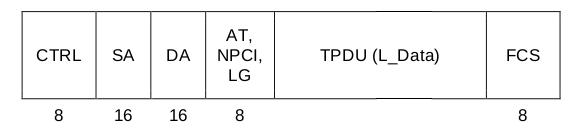
\includegraphics[width=0.5\textwidth]{figures/standardframe.png}
    \caption{Standard Frame}
    \label{fig:stdframe}
\end{figure}

\begin{figure}
    \centering
    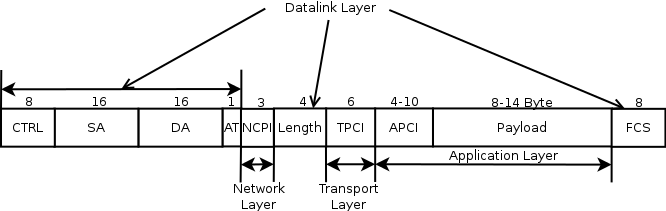
\includegraphics[width=0.5\textwidth]{figures/standardFrame.png}
    \caption{Standard Frame, in detail}
    \label{fig:stdFrameDetail}
\end{figure}

\begin{figure}
    \centering
    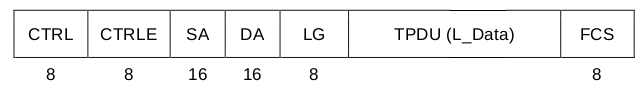
\includegraphics[width=0.5\textwidth]{figures/extendedframe.png}
    \caption{Extended Frame}
    \label{fig:extframe}
\end{figure}

\subsection{L\_Poll\_Data Frame}

These frames serve as data requests for a maximum of 15 bytes(payload of a standard
data frame) and start with a control field, as defined, followed by the 2 byte source address
of the sender(called Poll\_Data Master). The following 2 byte destination address is 
used to address up to 15 poll slaves, all belonging to the same poll group. The number of
exptected bytes and the check octet follow.

Poll requests are answered by poll slaves just by transmitting the databytes without any
special format, sent in the corresponding poll slave slot.

\subsection{Acknowledge Frame}

This frames are used to acknowledge request frames by just sending one byte representing
ACK, BUSY or NOT ACK.

\subsection{Network Layer}

\subsection{Transport Layer}

This layer provides services for reliable point-to-point connections, as well as connection-less point-to-point, 
point-to-domain(multicast) and point-to-all-points(broadcast):

\begin{itemize}
 \item point-to-point, connectionless\\T\_Data\_Individual: connection-less, unreliable point-to-point

 \item point-to-point, connection orientated:
 \\T\_Connect: establish reliable connection to individual address
 \\ 
 T\_Data\_Connected: send data over established connection
 \\ 
 T\_Disconnect: terminate connection to individual address 
 \\
 This service uses a timer to detect timeouts, and allows up to 3 retransmissions. Prior to sending data, a T\_Connect request has to be sent. If the
 remote device cannot handle a new connection, a T\_Disconnect request is returned to the sender. Otherwise, no confirmation or acknowledgment is sent
 to the remote device.
 
 \item point-to-multipoint, connectionless
 \\
 T\_Data\_Group: unreliable multicast to group address

 \item point-to-all-points, connectionless
 \\
 T\_Data\_Broadcast: unreliable broadcast to all devices of a domain

 \item point-to-all-points, connectionless
 \\
 T\_Data\_SystemBroadcast: unreliable broadcast to all devices of a domain FIXME: unterschied Broadcast-SystemBroadcast
\end{itemize}

\begin{figure}
    \centering
    \includegraphics[width=0.8\textwidth]{figures/"transport flags".png}
    \caption{Flags used at the Transport Layer}
    \label{fig:tFlags}
\end{figure}
%FIXME: quellenangabe bild, KNX standard

\subsection{Session Layer}

This layer is left empty in KNX and just forwards data transparently from the lower level to the upper level, and vice versa.

\subsection{Presentation Layer}

This layer is left empty in KNX and just forwards data transparently from the lower level to the upper level, and vice versa.

\subsection{Application Layer}

\subsection{Topologies}

TP1-64 allows up to 64, and TP1-256 up to 256 devices connected to one physical segment in
a linear, star, tree or mixed topology. The maximum distance between 2 devices in one
physical segment is 700m, with all devices in this segment sharing the logical address space
of a subnetwork. 

Up to 4 physical segments are combined by bridges to form lines, guaranteeing a galvanic separation
of these segments and extending the maximum allowed distance between devices, with a maximum
of 255 devices per line. While a bridge itself has no individual address, they acknowledge frames received 
and transmit them on the other side.

Theses lines itself can be combined by routers, forming so called areas, also providing a galvanic separation.

